---
title :   "The Linear Algebra behind a Truncated Series Approximation"
author:   "Rollen S. D'Souza"
date  :   "2020-12-30"
---
Most, if not all, engineering and applied mathematics students are familiar with the Fourier series.
Here I will give a slightly different treatment of the series.
It will have a similar flavour to that often seen in more formal mathematics classes that have covered it.
I will assume a fair knowledge of abstract linear algebra.

Define the set of functions
\[
  L_2([-1, 1])
    =
      \left\{
        f: [-1, 1] \to \mathbb{R}
        \;\middle|\;
        \int_{-1}^{1} (f(t))^2 ~dt < \infty
      \right\},
\]
where we'll take \(f\) to be integrable.
This space is an infinite-dimensional vector space over the field \(\mathbb{R}.\)
Given any two functions \(f,\) \(g\in L_2([-1, 1])\) define their inner product by
\[
  \langle f, g \rangle_{L_2} = \int_{-1}^{1} f(t) g(t)~dt.
\]
To avoid confusion, inner products over the space \(L_2([-1, 1])\) will always be subscripted with \(L_2.\)
Since \(\langle f, f \rangle\) is finite, the induced norm
\[
  \|f\|_{L_2} = \sqrt{\langle f, f \rangle_{L_2}}
\]
is well-defined.
%
Now let \(\mathbb{R}^{2n+1}\) have the usual inner product space structure.
The space \(\mathbb{R}^{2n+1}\) has a well-known orthonormal basis \(e_1, \ldots, e_{2n+1}.\)
Define a linear map \(M\) using this basis that satisfies
\[
  M(e_1) = 1
\]
and
\[
  M(e_{2k}) = \cos(k \pi t),\; M(e_{2k+1}) = \sin(k \pi t),\quad \forall 1\leq k\leq n.
\]
To this map \(M\) there exists an adjoint map \(M^*\) that satisfies, for all \(x \in \mathbb{R}^{2n+1}\) and \(f \in L_2([-1, 1]),\)
\[
  \langle M(x), f \rangle_{L_2}
  =
  \langle x, M^*(f) \rangle.
\]
A formula for \(M^*\) can be computed by writing both \(x\) and \(M^*(f)\) in terms of the orthonormal basis \(e_i.\)
In particular
\[
  M^*(e_i)
    =
      \frac{\langle 1, f \rangle_{L_2}}{\langle 1, 1\rangle_{L_2}} e_1
      +
      \sum_{k = 1}^{n}
        \frac{\langle \cos(k \pi t), f \rangle_{L_2}}{\langle \cos(k \pi t), \cos(k \pi t)\rangle_{L_2}}
        e_{2k}
        +
        \frac{\langle \sin(k \pi t), f \rangle_{L_2}}{\langle \sin(k \pi t), \sin(k \pi t)\rangle_{L_2}}
        e_{2k+1},
\]
which simplifies to
\[
  M^*(f)
    =
      \frac{1}{2}\langle 1, f \rangle_{L_2} e_1
      +
      \sum_{k = 1}^{n}
        \langle \cos(k \pi t), f \rangle_{L_2}
        e_{2k}
        +
        \langle \sin(k \pi t), f \rangle_{L_2}
        e_{2k+1}.
\]

Consider the following optimization problem.
%
\begin{quote}
  Given \(f \in L_2([-1, 1]),\) what is the \(x^* \in \mathbb{R}^{2n+1}\) that solves
  \[
    \min_{x \in \mathbb{R}^{2n+1}} \| M(x) - f \|_{L_2}^2.
  \]
\end{quote}
%
This question asks to find the coefficients \(x\) of our trignometric functions that best approximates the function \(f \in L_2([-1, 1])\) in terms of the distance function \(\|\cdot\|_{L_2}.\)
We can find an explicit expression for \(x^*.\)
This problem is just a linear least squares problem on a finite-dimensional vector space.
Most students will have encountered this problem in a linear algebra class.
The solution is directly computed by first computing the \href{https://en.wikipedia.org/wiki/Moore%E2%80%93Penrose_inverse}{Moore-Penrose pseudoinverse} of the matrix characterizing the problem.
We will take this approach.

Consider the linear map \(M^* \circ M: \mathbb{R}^{2n+1} \to \mathbb{R}^{2n+1}.\)
This is a linear map between finite-dimensional vector spaces which means it has a matrix representation.
We can say more.
Let \(x \in \mathbb{R}^{2n+1}\) be arbitrary and consider the inner product
\[
  \langle x, (M^* \circ M)(x) \rangle.
\]
Using the property of the adjoint, the above expression equals
\[
  \langle M(x), M(x) \rangle_{L_2}.
\]
This is positive if, and only if, \(M(x)\) is equal to a function whose square integral is zero.
The only way for \(M(x)\) to satisfy this is if \(x = 0\) since \(M\) is injective.
It follows that \(\langle x, (M^* \circ M)(x) \rangle > 0\) if, and only if, \(x \neq 0.\)
In coordinates, this is equivalent to saying
\[
  [x] \neq 0 \iff [x]^\top [M^*\circ M] [x] > 0.
\]
This demonstrates that the matrix \([M^* \circ M]\) is positive definite.
Positive definite matrices are invertible so \(M^* \circ M\) has a well-defined inverse.
Define
\[
  x^* = \left(M^* \circ M\right)^{-1}\left(M^*(f)\right).
\]
Compare with your sources to see that \((M^* \circ M)^{-1} \circ M^*\) is the (left) pseudoinverse.
I claim that this \(x^*\) is the solution to the optimization problem.

Skirting the proof here as it is a matter of second year linear algebra and calculus, what really is the value of this perspective?
Technically, not much besides the fact that we make explicit the fact that the standard (truncated) Fourier series \emph{is} the closest approximation of a function in terms of the standard inner product on \(L_2([-1, 1]).\)
Of course, this is something we already knew in advance.

Somewhat insignificantly, we explicitly used the fact that an orthogonal basis exists for the domain \(\mathbb{R}^{2n+1}\) --- for which we have a canonical choice --- rather than use the fact that the chosen basis of functions \(\cos\) and \(\sin\) are by themselves orthogonal with respect to this choice of inner product.
If we had instead started with a non-orthogonal set, one could either orthogonalize it using Gram-Schmidt or construct this left pseudoinverse.
Either method produces a solution to the ``best approximation'' problem.

Let us explore an example.
Consider the linear map \(M: \mathbb{R}^{2n +1} \to L_2([-1, 1])\) defined by
\[
  M(x) = \sum_{i = 1}^{2n+1} x^{i} t^{i-1} \in L_2([-1, 1]).
\]
Using the standard inner products on both spaces, the adjoint is defined as
\[
  M^*(f)
    = \sum_{i = 1}^{2n + 1} \langle f(t), t^{i-1} \rangle_{L_2} e_i
\]
Since \(M^* \circ M\) is a map between finite dimensional vector spaces, we can compute the element at row \(i\) and column \(j\) by computing the inner product
\[
  \langle e_i, (M^*\circ M)(e_j) \rangle = \langle M(e_i), M(e_j) \rangle_{L_2} = \langle t^{i - 1}, t^{j - 1} \rangle_{L_2}.
\]
That is, \(M^*\circ M\) in coordinates is the matrix of inner products between the basis elements \(t^k.\)
For example, when \(n = 5,\)
\[
M^* \circ M
  =
    \begin{bmatrix}
      2 & 0 & \frac{2}{3} & 0 & \frac{2}{5} & 0 & \frac{2}{7} & 0 & \frac{2}{9} & 0 & \frac{2}{11}\\ 0 & \frac{2}{3} & 0 & \frac{2}{5} & 0 & \frac{2}{7} & 0 & \frac{2}{9} & 0 & \frac{2}{11} & 0\\ \frac{2}{3} & 0 & \frac{2}{5} & 0 & \frac{2}{7} & 0 & \frac{2}{9} & 0 & \frac{2}{11} & 0 & \frac{2}{13}\\ 0 & \frac{2}{5} & 0 & \frac{2}{7} & 0 & \frac{2}{9} & 0 & \frac{2}{11} & 0 & \frac{2}{13} & 0\\ \frac{2}{5} & 0 & \frac{2}{7} & 0 & \frac{2}{9} & 0 & \frac{2}{11} & 0 & \frac{2}{13} & 0 & \frac{2}{15}\\ 0 & \frac{2}{7} & 0 & \frac{2}{9} & 0 & \frac{2}{11} & 0 & \frac{2}{13} & 0 & \frac{2}{15} & 0\\ \frac{2}{7} & 0 & \frac{2}{9} & 0 & \frac{2}{11} & 0 & \frac{2}{13} & 0 & \frac{2}{15} & 0 & \frac{2}{17}\\ 0 & \frac{2}{9} & 0 & \frac{2}{11} & 0 & \frac{2}{13} & 0 & \frac{2}{15} & 0 & \frac{2}{17} & 0\\ \frac{2}{9} & 0 & \frac{2}{11} & 0 & \frac{2}{13} & 0 & \frac{2}{15} & 0 & \frac{2}{17} & 0 & \frac{2}{19}\\ 0 & \frac{2}{11} & 0 & \frac{2}{13} & 0 & \frac{2}{15} & 0 & \frac{2}{17} & 0 & \frac{2}{19} & 0\\ \frac{2}{11} & 0 & \frac{2}{13} & 0 & \frac{2}{15} & 0 & \frac{2}{17} & 0 & \frac{2}{19} & 0 & \frac{2}{21}
    \end{bmatrix}
\]
This matrix is, in general, poorly conditioned.
It is recommended to construct an orthonormal basis of functions instead for this very reason.
In the case of polynomials, use the \href{https://en.wikipedia.org/wiki/Legendre_polynomials}{Legendre polynomials}.
It is easy to check that \(M^* \circ M\) is the identity map when the chosen basis is orthonormal.
The approximation of a bump function with \(2n + 1 = 11\) terms is displayed below.
%
\begin{figure}
  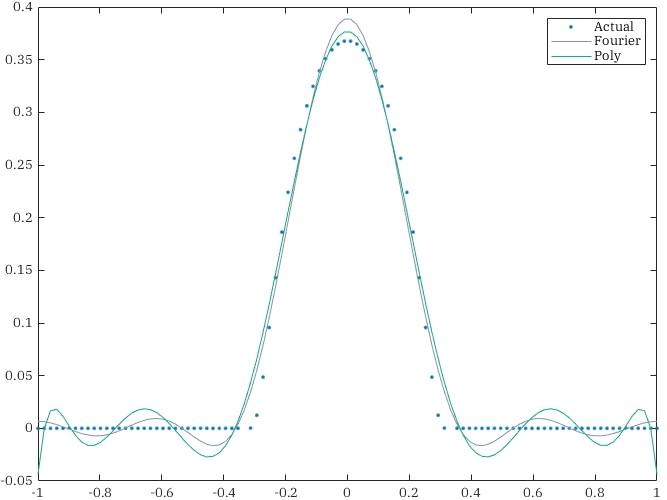
\includegraphics{/images/fourierseries/fourierpoly.png}
  \caption{Approxmation of a bump function with a truncated Fourier and polynomial series up to \(11\) terms.}
\end{figure}
%
